
\section{Theoretical Analysis}
\label{sec:analysis}
\subsection{Circuit frequency response}
With the equations below we determined the cut-off frequencies for the higher and lower cut-off frequencies. The former appears from the low-pass stage and the latter from the high pass stage.

\begin{equation}
w_L=\frac{1}{R_{1}C_{1}}
\end{equation}
\begin{equation}
w_H=\frac{1}{R_{2}C_{2}}
\end{equation}
This was the definition used to determine the central frequency, which is meant to be 1 kHz.
\begin{equation}
w_O=\sqrt{w_{H}w_{L}}
\end{equation}

\begin{table}[h!]
  \centering
  \begin{tabular}{|l|r|}
    \hline    
    {\bf Name} & {\bf Values} \\ \hline
    Lower Cut-Off Frequency & 723.431560 Hz \\ \hline 
Upper Cut-Off Frequency & 1446.863119 Hz \\ \hline 
Central Frequency & 1023.086723 Hz \\ \hline 
 
  \end{tabular}
  \caption{Cut off frequencies and central frequency.}
  \label{tab:data}
\end{table}

This central frequency result represents a 2.309\% relative error, which isn't a bad result considering the components used.

\begin{figure}[h!] \centering
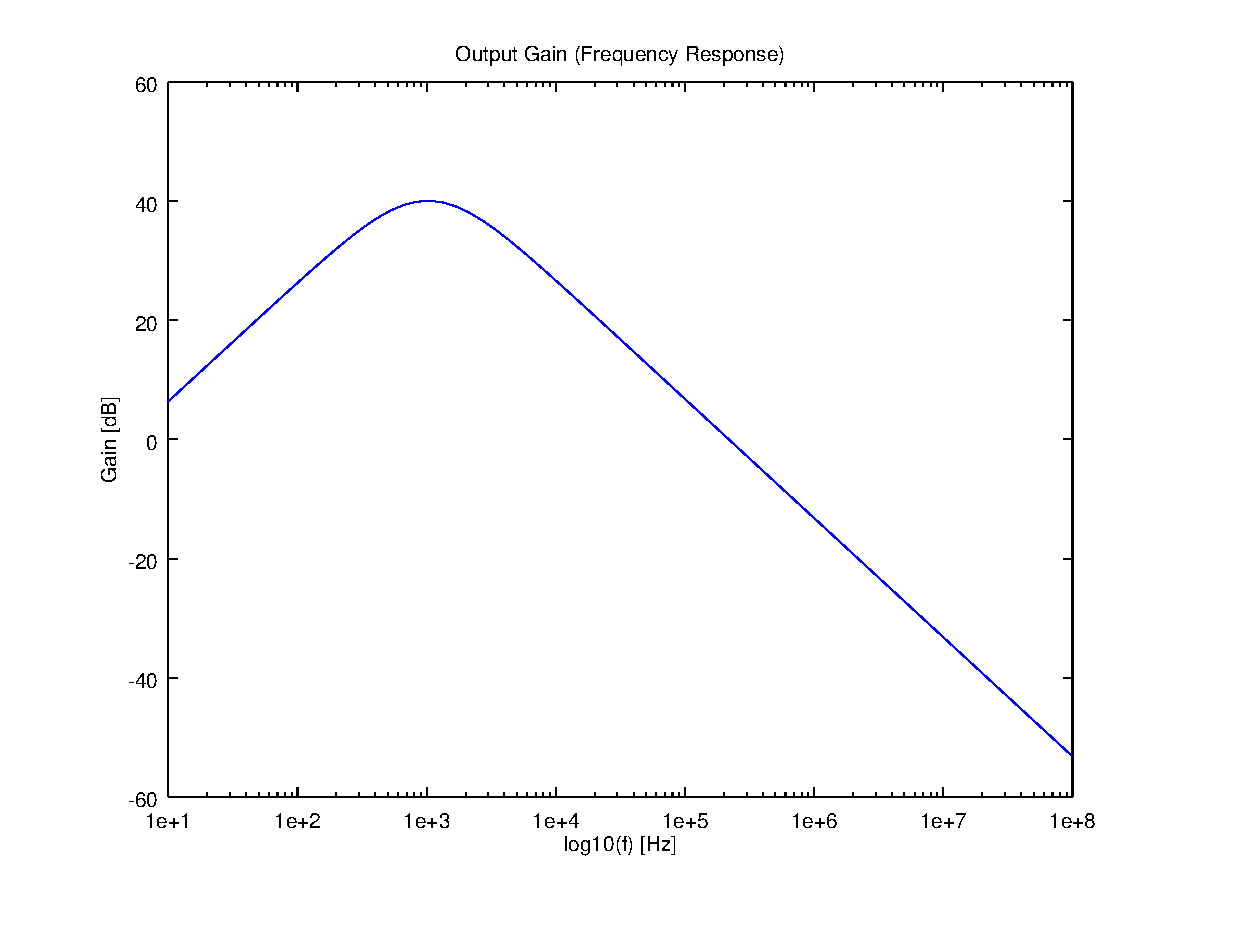
\includegraphics[width=0.6\linewidth]{gain.eps}
\caption{Voltage gain frequency response.}
\label{fig:gainfreq}
\end{figure}

As wanted, the plot has the trait of a narrower band-pass filter, with its top gain arriving in the 1 kHz neighbourhood, and the gain itself is on the 40 dB as pretended.

\begin{figure}[h!] \centering
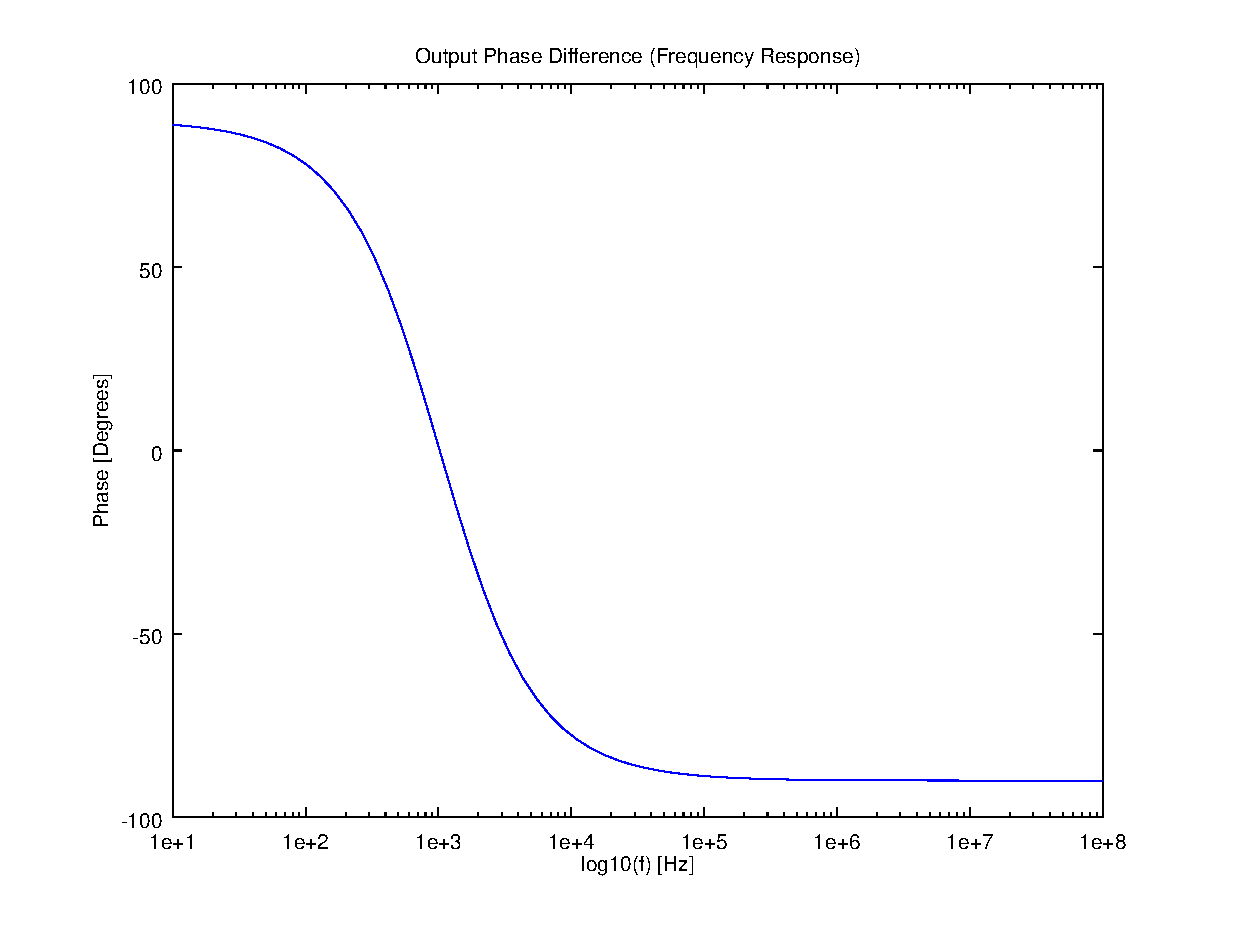
\includegraphics[width=0.6\linewidth]{phase.eps}
\caption{Voltage phase frequency response.}
\label{fig:gainfreq}
\end{figure}

The phase drops from 90 degrees to -90 degrees, which is cause of the 2 poles of the transfer function (which we will present in the next subsection), one pole introduced by the high-pass and the 
other pole introduced by the low pass. Each pole causes a 90 degree drop, 45º the decade before and 45º the decade after. At the central frequency, the phase is zero, which means the output 
voltage is in phase with the input voltage.

\subsection{Central frequency results}
For a frequency of 1 KHz we computed the circuit gain and input and output impedances for the amplifier. Also, we determined a theoretical figure of merit based on the predicted results with the set 
of values we chose.

The gain value for the entire circuit is obtained by multiplying the individual gains of each of the three stages of the circuit. This is an ideal situation, where we don't take into account the loss of signal between stages, or charge effects between the same stages.
These are the equations for the gain values:
\begin{equation}
High Pass Gain=|\frac{R_{1}C_{1}jw_{O}}{1+R_{1}C_{1}jw_{O}}|
\end{equation}
\begin{equation}
Amplifier Gain=1+\frac{R_{4}}{R_{3}}
\end{equation}
\begin{equation}
Low Pass Gain=|\frac{1}{1+R_{2}C_{2}jw_{O}}|
\end{equation}

Using the incremental model for the circuit (the input impedance of the OP-AMP is infinite and the output impedance of the OP-AMP is null, according to the model studied in class), we determined the following equations for the input and output impedances of the circuit:

\begin{equation}
Z_i = R_1 + \frac{1}{jw_{O}C_{1}}
\end{equation}
\begin{equation}
Z_o = \frac{R_2}{1+jw_OR_2C_2}
\end{equation}

\begin{table}[h!]
  \centering
  \begin{tabular}{|l|r|}
    \hline    
    {\bf Name} & {\bf Values} \\ \hline
    Gain (1 KHz) & 100.643363 \\ \hline 
Gain (1 KHz)(dB) & 40.055703 dB \\ \hline 
Gain (calculated central frequency) (dB) & 40.057714 dB \\ \hline 
$Z_{in}$ & 1000.000000 -723.431560j Ohm \\ \hline 
$Z_{in}$ modulus & 1234.241962 Ohm \\ \hline 
$Z_{in}$ phase & -35.883164 Degrees \\ \hline 
$Z_{out}$ & 676.732451 -467.723894j Ohm \\ \hline 
$Z_{out}$ modulus & 822.637497 Ohm \\ \hline 
$Z_{out}$ phase & -34.650304 Degrees \\ \hline 
Cost & 13626.952040MU \\ \hline 
Merit & 3.092445$*10^{-6}$ \\ \hline 
 
  \end{tabular}
  \caption{Gain, input and output impedances at the central frequency.}
  \label{tab:data}
\end{table}

This way we can see that the gain for a frequency of 1KHz is almost the same as the gain for the calculated central frequency, meaning the 1KHz frequency is still very much within the band pass region.
We obtained then a relative error of 0.643\% for the gain at central frequency, which is meant to be 100, so this a 
fantastic theoretical result. The input impedance value is quite high, which is good, so, depending on the resistance of the input, most of the input 
voltage will flow through ahead to the OP-AMP as pretended. The output impedance value though is quite large, so this circuit will not be suited to loads with very low resistance values, but given 
the components we had available there wasn't much room for improvement. Also, we don't know the load that would be linked to this circuit, so we can't fully know how good or bad this value is, 
we just know it is clearly not the most desirable.
